\chapter{Introduction}\label{chap:01}

\section{Motivation}
In difference to products, which can be manufactured and stored, is a service volatile.
A service is simultaneously produced or rather provided by the \emph{service provider} and consumed by the \emph{customer}.
A typical example is a \emph{telecommunication service} like speech telephony, or Internet access.
%US Communications Act 1934
Telecommunication services provide communication, \ie, data transmission, between one or more parties.
Here a party can be a person but also a computer.
A service provider maintains the network infrastructure to provide those services and makes it available to potential users\footnote{Throughout this a person engaging a service is called \emph{user} of this service without distinction if he is the actual customer.}.
The actual service is produced, when a user uses a provided service, using the provider's network infrastructure for data transmission.

As a service is produced when it is used, the \emph{service performance} might be varying.
Here, service performance are absolutely measurable parameters of this service like transmission bandwidth and one-way transmission delay~\citep[\cf,][p. 12]{moller_assessment_2000}.
In case of a telecommunication service varying service performance can be the result of current network load conditions, network equipment failure, but also related to end-user devices (\eg, the telephone) and other factors.
Usage of telecommunication services can be divided into two aspects.
First, a user can actively interact with a service like starting and engaging a telephone conversation.
Second, user can passively use a service, \eg, reachability of a telephone.

The active use by a user of a telecommunication service also results in a \emph{perceived quality} of this interaction.
It is assumed that perceived quality results from a comparison between the \emph{desired experience} and \emph{actual experience}. %Expected experience?
Here experience includes all perceptions resulting from this service instance \citep[\cf,][p.13]{Book chapter 2}.
The perceived quality of an interaction with a service is affected by the experienced service performance, but also individual factors like requirements, tasks, etc.

%QoE Methods; human perception 
Understanding the relationship between service (or system) performance with perceived quality has become important field of research investigated the so-called \ac{QoE}.
Starting from speech transmission for telephony \citep[\cf,][]{IEEE Recommended Practice for Speech Quality Measurements} and the resulting degradations, \ac{QoE} now mainly considers digital transmission of multimedia data \citep{moller_quality_2014}.
This includes the production, coding, transmission, decoding and reproduction of text, voice, speech, image and video information.
Specific characteristics of human perceptual system have been used to develop enhanced coding mechanisms like \ac{MP3} or \ac{H.264}, which use lossy compression to provide a reduction in data rate while provide only little reduction in perceived quality.

Another application of knowledge about perceived quality is the monitoring of network transmission infrastructure.
This allows to estimate the actual impact of degradations on a user and enable service provider to react accordingly to avoid severe reductions the perceived quality.
In case of a video streaming service for example a temporary reduction in network bandwidth, the actual impact leading to stalling could be avoided by a reduction of encoding bandwidth, frame rate, or resolution.
Although perceived quality is likely to be affected the service is still provided and remains useful for the user.

%Service choice
In general a user can chose from a variety of service providers, which provide a similar service, and select the one provider that suits best.
For a reasoned selection a user must know his needs, requirements, economical limits and estimate the perceived quality (\ie, \emph{assumed quality}).
Based upon this knowledge he can estimate, if usage of a service is likely to be satisfying for him.
After using and experiencing a service, the user can then decide, if this service fulfills his needs, also including perceived quality, and if he might use it again, or rather select a different service provider the next time he needs this type of service \citep[\cf,][]{geerts_linking_2010}.
%Hygenic factor?

\section{Research Questions}
This work extends prior work by investigating the impact of varying service performance on the perceived quality, when the one or more service(s) are used repeatedly.
This is, in fact, a common case for telecommunication service(s).
For example a user of a mobile  provider will use the provided service(s) usually repeatedly as his telephone number is bound to the service provider.

Especially for a telecommunication service the performance might be varying from usage instance to usage instance.
Although some prior work has been done on varying performance during one usage episode, it is so far not known how perceived quality evolves over several distinct episodes.
This, however, is expected one factor contributing to \emph{service quality} \citep[\cf,][]{zeithaml_behavioral_1996}.
The construct service quality maintains a holistic view from a business perspective of service usage and is important for economical decisions.
%In fact, perceived quality is an implicit part of service quality.

In this thesis I investigate perceived quality over several distinct and meaningful interactions with a service.
Such an interaction is denoted as \emph{episode} (\cf, \autoref{chap:03}) and the perceived quality over several usage episodes is denoted as \emph{multi-episodic perceived quality}. % (\cf, \autoref{img:chap01:multi-episodic}).
I focus on telecommunication services(s) as those are well-studied with regard to perceived quality, are widely used and degradations, irrespective of the actual reason, occur relative frequently.

In this thesis I address one research question: \\
\begin{itemize}
\item How does multi-episodic quality for one user evolve over several usage episodes with the one service and which factors determine the multi-episodic quality?
%\item How is multi-episodic perceptual quality affected, if different services are used, and how are those quality judgments integrated to form an overall judgment?
\end{itemize}

%\begin{figure}
%	\centering
%	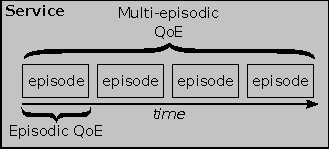
\includegraphics[width=0.6\columnwidth]{figure/multi-episodic}
%	\caption{Repeated usage episodes with one service and their episodic perceived quality form a multi-episodic perceived quality in the user.}
%	\label{img:chap01:multi-episodic}
%\end{figure}

%Memory
Each usage episode has a perceived quality, which can be assessed momentary while in the usage episode and also in retrospective after the usage episode is finished.
Multi-episodic perceived quality requires experiencing multiple usage episodes with a service, but unknown how this the integration of prior experiences occurs.
It could be a continuous process that integrates current experiences immediately into a current view, a retrospective assessment evaluating all memorized and recallable information, or a mixture of both.

%TODO: NAME time-frames! hour, days and also weeks.
\section{Goals}
In this thesis I pursue two goals towards understanding multi-episodic perceived quality.
In fact, the development of multi-episodic perceived quality cannot be observed directly (\cf, \autoref{chap:02}) and therefore multi-episodic perceived quality can only sampled resulting in a judgment of the multi-episodic perceived quality.

\paragraph*{Goal 1}
I will investigate how episodic quality affects multi-episodic judgments.

\paragraph*{Goal 2}
I will investigate how multi-episodic judgments can be predicted based upon episodic judgments.

\section{Structure}
This thesis is divided into two parts.
In \emph{Part I} I introduce concepts and fundamentals that form the basis for my approach towards multi-episodic perceived quality.
In \autoref{chap:02} an introduction on \ac{QoE} is given.
This includes prior work on psychophysics, perception and the quality formation process.
At the end of this chapter the relationship to higher level concepts like satisfaction and service quality is discussed.
In \autoref{chap:03} I present relevant concepts that affect recall and thus retrospective judgments of a \emph{general experience}.
Here, I will discuss how memory affects retrospective judgments and present known temporal effects from related fields.
In \autoref{chap:04} I present the state of the art on performance fluctuations on \ac{QoE} in one episode.
This chapter closes with a review on found temporal effects in this domain and how those effects are modeled.
This part closes with an overview on prior work on multi-episodic perceived quality (\autoref{chap:05}).
Here the assessment methodology developed by \cite{moller_single-call_2011}, which is the following denoted as \emph{defined use}, is presented in detail.

In \emph{Part II} I present my work towards multi-episodic perceived quality based upon the defined use methodology.
In \autoref{chap:towards} I describe the hypotheses I investigated with all necessary details.
In \autoref{chap:lab} I present my work on multi-episodic perceived quality in time-frame of up to one hour.
Those studies and the found results are then complemented in \autoref{chap:field} with studies on multi-episodic perceived quality over several days.
In \autoref{chap:modeling} the prediction models for multi-episodic perceived quality are implemented presented.
\autoref{chap:discussion} summarizes the thesis, discusses the results and highlights direction for future work.
